\subsection{Tworzenie nowych typów danych}

Funkcjonalność tworzenia nowych typów danych nie wyróżnia przygotowanego systemu
od systemów CMS dostępnych na rynku. Jest zaimplementowana, jako lista
formularzy. Każdy formularz odpowiada jednej kolumnie w nowo utworzonej tabeli.
Administrator może dodawać nowy formularz, lub kasować już istniejący.

Pojedyńczy formularz zawiera następujące elementy:

\begin{itemize}

    \item Pole tekstowe, gdzie administrator podaje nazwę kolumny.

    \item Menu rozwijane pozwalające na wybór typu kolumny.

    \item Pole wyboru, które pozwala określić administratorowi, czy kolumna może
    zawierać wartości \verb|null|.

    \item Pole wyboru, które pozwala określić czy kolumna posiada wartość
    domyślną wraz z polem tekstowym, które pojawia się, gdy administrator
    oznaczy kolumnę jako posiadającą wartość domyślną, gdzie należy podać
    wartość domyślną.

\end{itemize}

Pod listą formularzy można znaleźć przycisk umożliwiający wysłanie definicji
tabeli do programu backend, który utworzy ją w bazie danych. Pod przyciskiem
znajduje się ramka, w której pojawiają się możliwe błędy zwrócone przez bazę
danych, lub informacja o pomyślnym stworzeniu tabeli.

Interfejs tworzenia nowych typów danych jest pokazany na rysunku
\ref{tableCreationFigure}.

\begin{figure}[h]
    \centering
    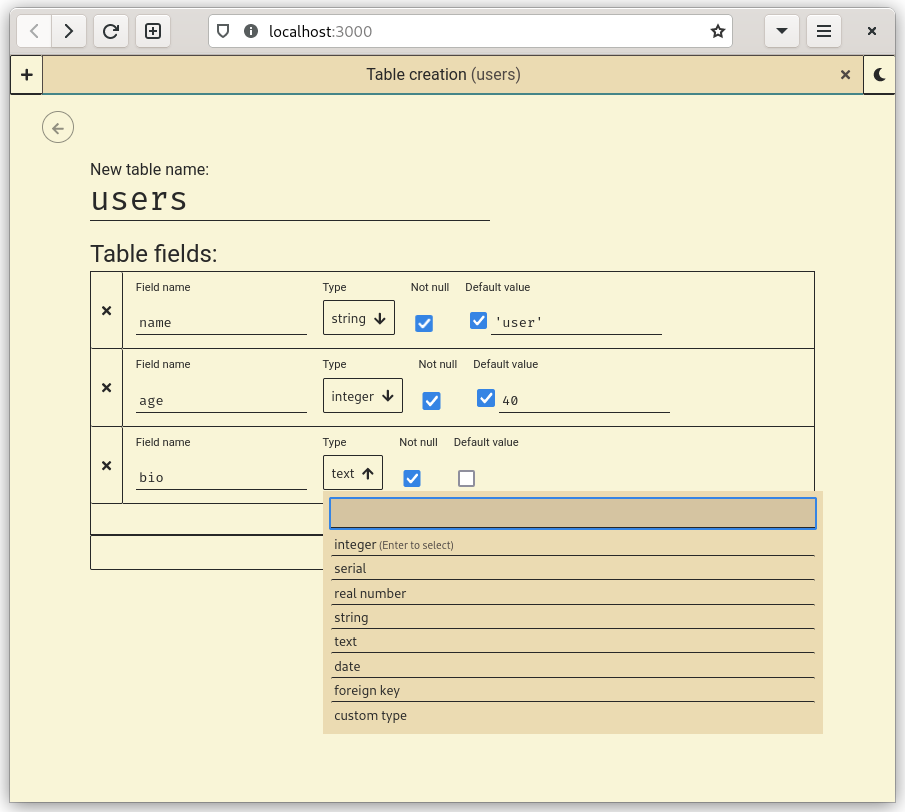
\includegraphics[width=0.8\textwidth]{./img/table_creation.png}
    \caption{Interfejs tworzenia nowego typu danych}
    \label{tableCreationFigure}
\end{figure}

\subsection{Zarządzanie danymi}

Interfejs zarządzania danymi zawiera menu rozwijane, które administrator używa
do wyboru tabeli, której danymi chce zarządzać. Komponent używany do tego menu
to ten sam komponent, który jest użyty do wyboru typu danych w interfejsie
tworzenia nowych typów danych.

Pierwszym elementem, który administrator zauważy po wybraniu tabeli jest
formularz wprowadzania nowych danych. Składa się on z listy formularzy,
podobnie, jak interfejs tworzenia nowych typów danych. Aplikacja dobiera
odpowiedni typ formularza HTML do typu danych kolumny, której dane daje
możliwość wprowadzania. Przykładowo, kolumny typu \verb|varchar| spowodują
wyświetlenie elementu \verb|<input type="text">|, elementy typu \verb|text|
spowodują wyświetlenie elementu \verb|<textarea>|, a kolumny typu \verb|date|
spowodują wyświetlenie elementu \verb|<input type="date">|.

Funkcją, na którą warto zwrócić uwagę jest wyświetlanie ostrzeżenia, przy próbie
wprowadzenia danych niedomyślnych do kolumny, która jest kluczem głównym, i
której wartość domyślna zawiera \verb|nextval|. Może to spowodować błąd w
późniejszej próbie dodania danych do tej tabeli przez powtórzenie klucza
głównego.

Pod interfejsem wprowadzania nowych danych znajduje się widok danych w tabeli.
Widok ten zawiera funkcje zmiany sortowania, edycji oraz usuwania danych.
Interfejs wspiera paginację, domyślnie wyświetla sto rzędów.

Interfejs jest pokazany na rysunku \ref{tableDataManagementFigure}.

\begin{figure}[h]
    \centering
    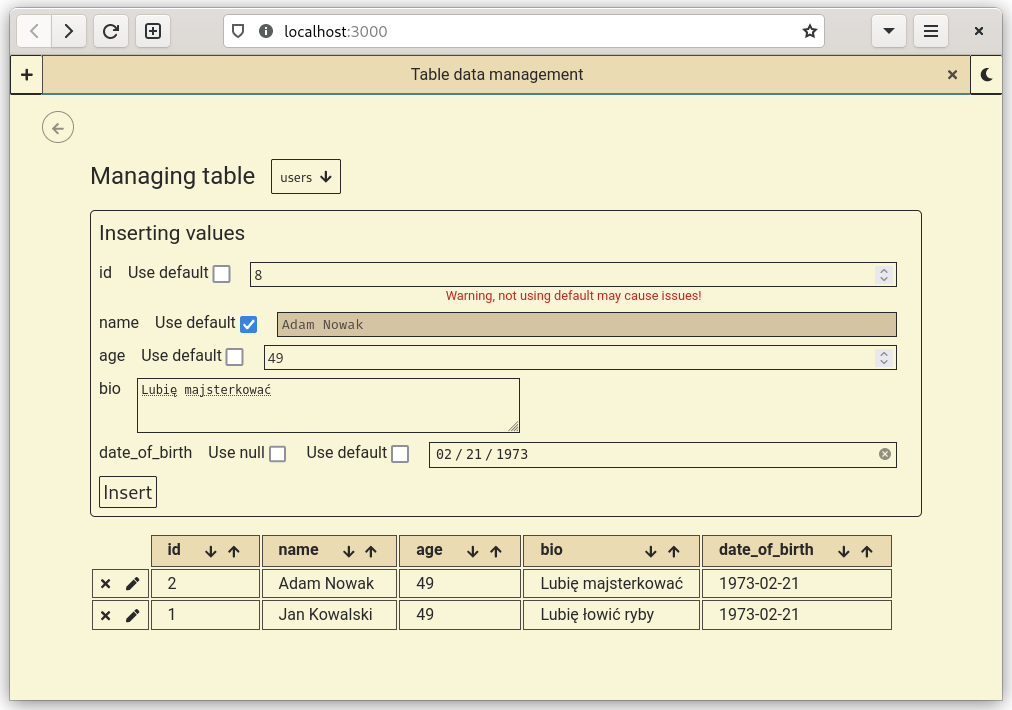
\includegraphics[width=\textwidth]{./img/table_data_management.png}
    \caption{Interfejs zarządzania danymi w tabeli}
    \label{tableDataManagementFigure}
\end{figure}

